
\documentclass[fleqn,a4paper,12pt]{article}

% fleqn to left align equations
%\setlength{\textwidth}{2in}
\usepackage{hyperref}
\usepackage{fancyhdr}
\usepackage{enumitem}
%\renewcommand{\familydefault}{\rmdefault}
\renewcommand{\familydefault}{\sfdefault}
%\usepackage{helvet}
%\pagestyle{fancy}
\date{}
%\pagenumbering{gobble}
\usepackage{geometry}
\pagenumbering{gobble}
\usepackage{multicol}
\usepackage{tikz}
\usepackage{amsmath}
\usepackage{amsfonts}
\usepackage{mathtools,xparse}
\usepackage{listings}
\usepackage{amssymb}
\usepackage{float}


%\fancyhf{}
%\pagestyle{fancy}
%\rhead{Mina Jafari}
%\lhead{ML-HW1}
\newcommand{\norm}[1]{\left\lVert#1\right\rVert}

%Abernethy
\newcounter{probnum}
\newcounter{subprobnum}
\newcounter{subsubprobnum}
\stepcounter{probnum}
\stepcounter{subprobnum}
\stepcounter{subsubprobnum}

\newcommand{\nsubprob}[2]{\addtolength{\leftskip}{-3em}\vspace{0em} \noindent \textbf{ \noindent #1) \stepcounter{subprobnum}} #2\par \addtolength{\leftskip}{3em}}

\def \probmargin{1.2em}
\def \probvspace{0em}

\newcommand{\nprob}[2]
{
	
	\vspace{\probvspace}
	\setcounter{subprobnum}{1}
	\setlength{\leftskip}{0em}
	\noindent \arabic{probnum}) \textbf{#1. } #2 
	\vspace{\probvspace}
	\stepcounter{probnum}
}

\newcommand{\subprob}[1]
{
	
	\setlength{\leftskip}{\probmargin}
	\setcounter{subsubprobnum}{1}
	
	\def \subttl{\textbf{(\alph{subprobnum}) }}
	\settowidth{\parindent}{\subttl}
	\addtolength{\leftskip}{\parindent}
	\setlength{\parindent}{-\parindent}
	\subttl #1
	\stepcounter{subprobnum}
	\vspace{\probvspace}
	\setlength{\parindent}{0em}
	
}

\newcommand{\subsubprob}[1]
{
	
	\setlength{\leftskip}{\probmargin}
	\addtolength{\leftskip}{\probmargin}
	
	\def \subttl{\textbf{(\roman{subsubprobnum}) }}
	\settowidth{\parindent}{\subttl}
	\addtolength{\leftskip}{\parindent}
	\setlength{\parindent}{-\parindent}
	\subttl #1
	\stepcounter{subsubprobnum}
	\vspace{\probvspace}
	\setlength{\parindent}{0em}
	
}
%end-abernethy

\geometry{a4paper,left=20mm,right=20mm,top=20mm,bottom=20mm}
%\renewcommand{\headrulewidth}{1.5 pt}

\hypersetup
{
    pdfauthor={Mina Jafari},
    pdfsubject={Homework2},
    pdftitle={MachineLearning},
    pdfkeywords={ML-HW2}
}
\linespread{1.0}

\makeatletter
\newcommand{\hwclass}[1]{\def \TVclass{#1}}
\newcommand{\hwdue}[1]{\def \TVdue{#1}}
\newcommand{\hwassignment}[1]{\def \TVassignment{#1}}
\makeatother

% Title Heading
\renewcommand{\maketitle}
{
	\begin{center}
		\newlength{\titlerulewidth}
		\def \hmwkttl{{\TVclass\, - \TVassignment}}
		\settowidth{\titlerulewidth}{\hmwkttl}
		
		\rule{\titlerulewidth}{1pt}\\[3mm]
		\hmwkttl \\[3mm]
	%	\makebox[\titlerulewidth]{\small \TVname \hspace{1em} \hfill \hfill  group member: Joshua Kammeraad} \\
		\makebox[\titlerulewidth]{\small \TVname \hspace{1em}} \\
		\makebox[\titlerulewidth]{\footnotesize {group member: Joshua Kammeraad} \hspace{1em}} \\
		\rule{\titlerulewidth}{1pt}\\[3mm]
	\end{center}
	
	\vspace{3em}
}

\def\TVname{Mina Jafari}

\hwclass{EECS 545 -- Machine Learning}
\hwdue{11:00pm 03/21/2016}
\hwassignment{Homework \#4}
\begin{document}
\maketitle	

\nprob{Question 1}{

\subprob{}{
	\begin{flalign*}
	    I(X, Y) &= -\int\int p(x,y)\ln \frac{p(x)p(y)}{p(x,y)} dxdy\\
			    &= -\int\int p(x,y)\ln (p(x)p(y)) dxdy + \int\int p(x,y)\ln p(x,y) dxdy\\
			    &= -\int\int p(x,y)\ln (p(x)p(y)) dxdy + \int\int p(x,y)\ln (p(x\vert y)p(y)) dxdy\\
			    &= -\int\int p(x,y)\ln p(x) dxdy - \int\int p(x,y)\ln p(y) dxdy\\
			    &+ \int\int p(x,y)\ln p(x\vert y) dxdy + \int\int p(x,y)\ln p(y) dxdy\\
			    &= H(X) - H(X | Y)\\
		I(X, Y) &= -\int\int p(x,y)\ln \frac{p(x)p(y)}{p(x,y)} dxdy\\
			    &= -\int\int p(x,y)\ln (p(x)p(y)) dxdy + \int\int p(x,y)\ln p(x,y) dxdy\\
			    &= -\int\int p(x,y)\ln (p(x)p(y)) dxdy + \int\int p(x,y)\ln (p(y\vert x)p(x)) dxdy\\
			    &= -\int\int p(x,y)\ln p(x) dxdy - \int\int p(x,y)\ln p(y) dxdy\\
			    &+ \int\int p(x,y)\ln p(y\vert x) dxdy + \int\int p(x,y)\ln p(x) dxdy\\
			    &= H(Y) - H(Y | X)
	\end{flalign*}
	}
	
\subprob{}{
	\begin{flalign*}
		I(X, Y) &= H(X) - H(X | Y) = H(X) - H(f(Y) | Y) = H(X)\\
		I(X, Y) &= H(Y) - H(Y | X) = H(Y) - H(f(X) | X) = H(Y)\\
	\end{flalign*}
	}
		
\subprob{}{
	\begin{flalign*}
	\end{flalign*}
	}

\subprob{}{
	\begin{flalign*}
		&H[x] = -\int_{}^{}p(x)\ln p(x)dx\\
		&\int_{-\infty}^{\infty}p(x)dx = 1, \text{    } \int_{-\infty}^{\infty}xp(x)dx = \mu, \text{    } \int_{-\infty}^{\infty}(x-\mu)^2 p(x)dx = \sigma^2\\
		&\mathcal{L}(x, \lambda_1, \lambda_2, \lambda_3) = -\int_{-\infty}^{\infty}p(x)\ln p(x)dx + \lambda_1 \left( \int_{-\infty}^{\infty}p(x)dx - 1 \right) + \lambda_2 \left( \int_{-\infty}^{\infty}xp(x)dx - \mu \right)\\
		&+ \lambda_3 \left( \int_{-\infty}^{\infty}(x-\mu)^2 p(x)dx - \sigma^2 \right)\\
		&\frac{\partial }{\partial p(x)} \mathcal{L}(x, \lambda_1, \lambda_2, \lambda_3) = -\ln p(x) - 1 + \lambda_1 + \lambda_2 x + \lambda_3(x-\mu)^2 = 0\\
		&\implies p(x) = \exp\left( -1+\lambda_1+\lambda_2x+\lambda_3(x-\mu)^2 \right)\\
		&\text{using Mathematica to solve the integrals:}\\
		&\implies \lambda_1 = 1-\frac{1}{4}\ln (4\pi^2\sigma^4), \lambda_2=0, \lambda_3 = \frac{-1}{2\sigma^2}\\
		&\implies p(x)=\exp \left( -1+1-1/4 \ln (4\pi^2\sigma^4) + 0+ \frac{-(x-\mu)^2}{2\sigma^2} \right)\\
		&=\frac{1}{(2\pi\sigma^2)^{1/2}} \exp\left( \frac{-(x-\mu)^2}{2\sigma^2} \right)\\
		&\frac{\partial^2 H[x]}{\partial p(x)^2} = \frac{\partial^2 (-p(x)\ln p(x))}{\partial p(x)^2} = \frac{-1}{p(x)}, \text{    } 0 < p(x) \leq 1\\
		&\implies H^{''}[x] \text{is concave and Gaussian is the maximum entropy distribution} \implies H(q) \leq H(p)
	\end{flalign*}
%	\begin{figure}[!ht]
%		\centering
%		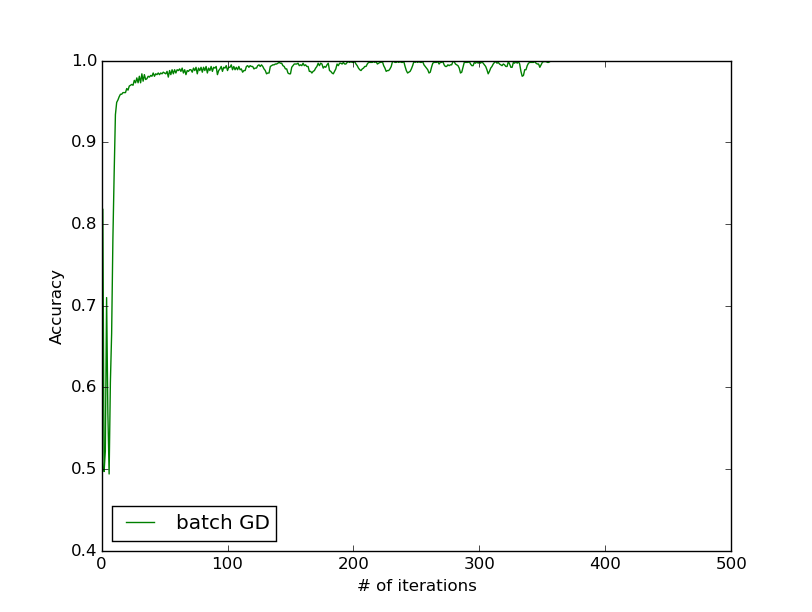
\includegraphics[width=0.5\textwidth]{question-1/1-d.png}
%	\end{figure}
%	\lstinputlisting[language=Python, basicstyle=\scriptsize]{question-1/q1-d.py}
	}
}
\vspace{15cm}
\nprob{Question 2}{
	
\subprob{}{
	\begin{flalign*}
		\text{Dirichlet}(\mathbf{p} | \mathbf{\alpha}) &= \frac{\Gamma(\sum_{k=1}^m \alpha_k)}{\prod_{k=1}^m \Gamma(\alpha_k)} \prod_{k=1}^m p_k^{\alpha_k - 1}\\
		B &= \frac{\Gamma(\sum_{k=1}^m \alpha_k)}{\prod_{k=1}^m \Gamma(\alpha_k)}\\
		\text{Dirichlet}(\mathbf{p} | \mathbf{\alpha}) &= \exp \big[ \log B + \sum_{k=1}^{m} (\alpha_k - 1) \log p_k \big]\\
													   &= \exp \big[ \log B + \eta(\alpha)^{\top} T(\mathbf{p}) \big]\\
													   &= \exp \big[ \eta(\alpha)^{\top} T(\mathbf{p}) - A(\alpha) \big]\\
													   &\eta(\alpha) = (\alpha_k - 1)\\
													   & T(\mathbf{p}) = \log p_k\\
													   & A(\alpha) = \log\frac{1}{B}
	\end{flalign*}
}

\subprob{}{
	\begin{flalign*}
		F(\alpha) &= \log P(\mathcal{D} | \alpha)\\
				  &= \log \prod_{j=1}^{N} p(p^j \vert \alpha) = \log \prod_{j=1}^{N} \frac{\Gamma(\sum_{k=1}^m \alpha_k)}{\prod_{k=1}^m \Gamma(\alpha_k)} \prod_{k=1}^m (p_k^j)^{\alpha_k - 1}\\
				  &= \sum_{j=1}^{N} \bigg[ \log \frac{\Gamma(\sum_{k=1}^m \alpha_k)}{\prod_{k=1}^m \Gamma(\alpha_k)} + \sum_{k=1}^m (p_k^j)^{\alpha_k - 1} \bigg]\\
				  &= \sum_{j=1}^{N} \bigg[ \log \Gamma(\sum_{k=1}^m \alpha_k) - \sum_{k=1}^{m} \log \Gamma(\alpha_k) + \sum_{k=1}^m (\alpha_k-1) \log p_k^j \bigg]\\
				  &= N \bigg[ \log \Gamma(\sum_{k=1}^m \alpha_k) - \sum_{k=1}^{m} \log \Gamma(\alpha_k) + \frac{1}{N}\sum_{k=1}^m (\alpha_k-1) \sum_{j=1}^{N}\log p_k^j \bigg]\\
				  &= N \bigg[ \log \Gamma(\sum_{k=1}^m \alpha_k) - \sum_{k=1}^{m} \log \Gamma(\alpha_k) + \sum_{k=1}^m (\alpha_k-1) \hat{t}_k \bigg]
	\end{flalign*}
}

\subprob{}{
	\begin{flalign*}
		\frac{\partial F}{\partial \alpha_i} &= \frac{\partial}{\partial \alpha_i}N \bigg[ \log \Gamma(\sum_{k=1}^m \alpha_k) - \sum_{k=1}^{m} \log \Gamma(\alpha_k) + \sum_{k=1}^m (\alpha_k-1) \hat{t}_k \bigg]\\
		&= N \bigg[ \frac{\Gamma'(\sum_{k=1}^m \alpha_k)}{\Gamma(\sum_{k=1}^m \alpha_k)} - \frac{\Gamma'(\alpha_i)}{\Gamma(\alpha_i)} + \hat{t}_k \bigg]\\
		&= N \bigg[ \Psi(\sum_{k=1}^m \alpha_k) - \Psi(\alpha_i) + \hat{t}_k \bigg]
	\end{flalign*}
}

\subprob{}{
	\begin{flalign*}
		H &\triangleq \nabla_{\alpha}^2 F(\alpha) = \frac{\partial^2 F}{\partial \alpha_i \partial \alpha_j} = \frac{\partial}{\partial \alpha_j} \frac{\partial F}{\alpha_i}\\
		  &=\frac{\partial}{\partial \alpha_j} N \bigg[ \Psi(\sum_{k=1}^m \alpha_k) - \Psi(\alpha_i) + \hat{t}_k \bigg]\\
		  &= N \bigg[ \Psi'(\sum_{k=1}^m \alpha_k) - \delta_{ij} \Psi'(\alpha_i) \bigg]\\
		  &= Q + c11^T\\
		  & q_{ij} =  - N \delta_{ij} \Psi'(\alpha_i), \text{  } 
		  \delta_{ij} = \begin{cases}
		  0,& \text{if } i \neq j\\
		  1,& \text{if } i = j
		  \end{cases}\\
		  & c = N \Psi'(\sum_{k=1}^m \alpha_k)
	\end{flalign*}
}

\subprob{}{
	\begin{flalign*}
		\alpha^{new} &= \alpha^{old} - \big[ H_F(\alpha^{old}) \big]^{-1} \cdot \nabla F(\alpha^{old})\\
					 &= \alpha^{old} - \big[ Q + c11^T \big]^{-1} \cdot \nabla F(\alpha^{old})\\
					 &= \alpha^{old} - \big[ Q^{-1} - \frac{Q^{-1} \cdot 1 \cdot 1^{\top} Q^{-1}}{\frac{1}{c} + 1^{\top} \cdot Q^{-1} \cdot 1} \big] \cdot \nabla F(\alpha^{old})\\
					 & \nabla F(\alpha) =
					 \begin{bmatrix}
					 \frac{\partial F}{\partial \alpha_1}\\[0.6em]
					 \frac{\partial F}{\partial \alpha_2}\\[0.6em]
					 \vdots\\[0.6em]
					 \frac{\partial F}{\partial \alpha_m}\\[0.6em]
					 \end{bmatrix}
	\end{flalign*}
}

\subprob{}{
	\begin{figure}[H]
		\centering
		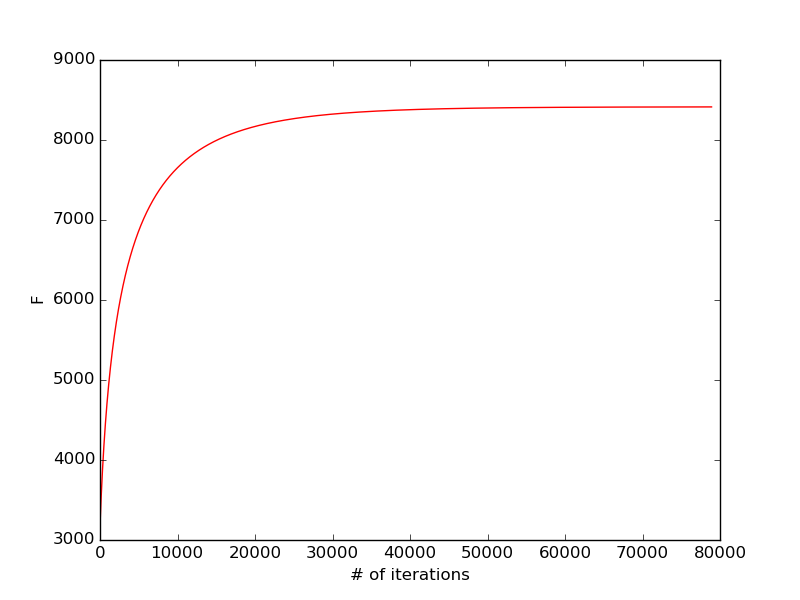
\includegraphics[width=0.6\textwidth]{question-2/plot-1.png}
		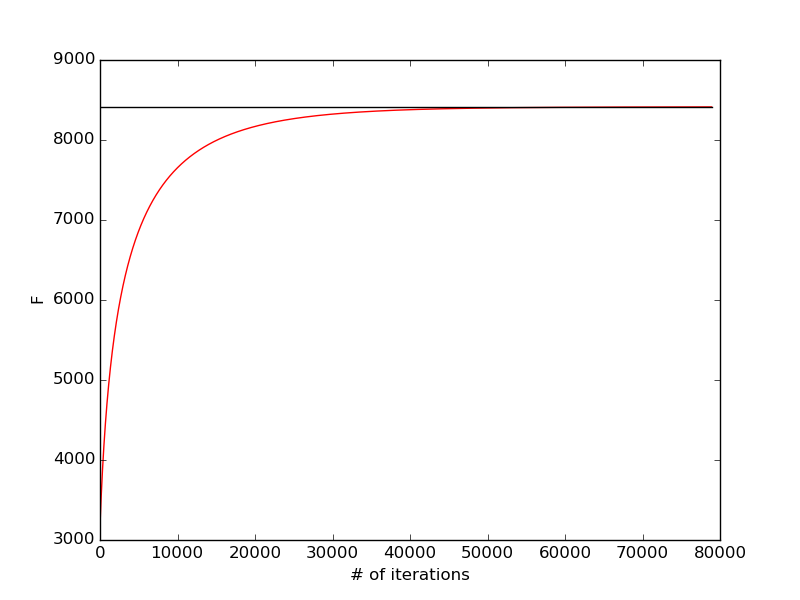
\includegraphics[width=0.6\textwidth]{question-2/plot-2.png}
	\end{figure}
	
	$\alpha$ = [9.96873078, 4.9528229, 14.60503616, 19.4465898, 48.57156412]
	
	\lstinputlisting[language=Python, basicstyle=\scriptsize]{question-2/hw4p2.py}
	}
}

\vspace{10cm}
\nprob{Question 3}{
	\subprob{}{
		\subsubprob{}{
				\begin{figure}[H]
					\centering
					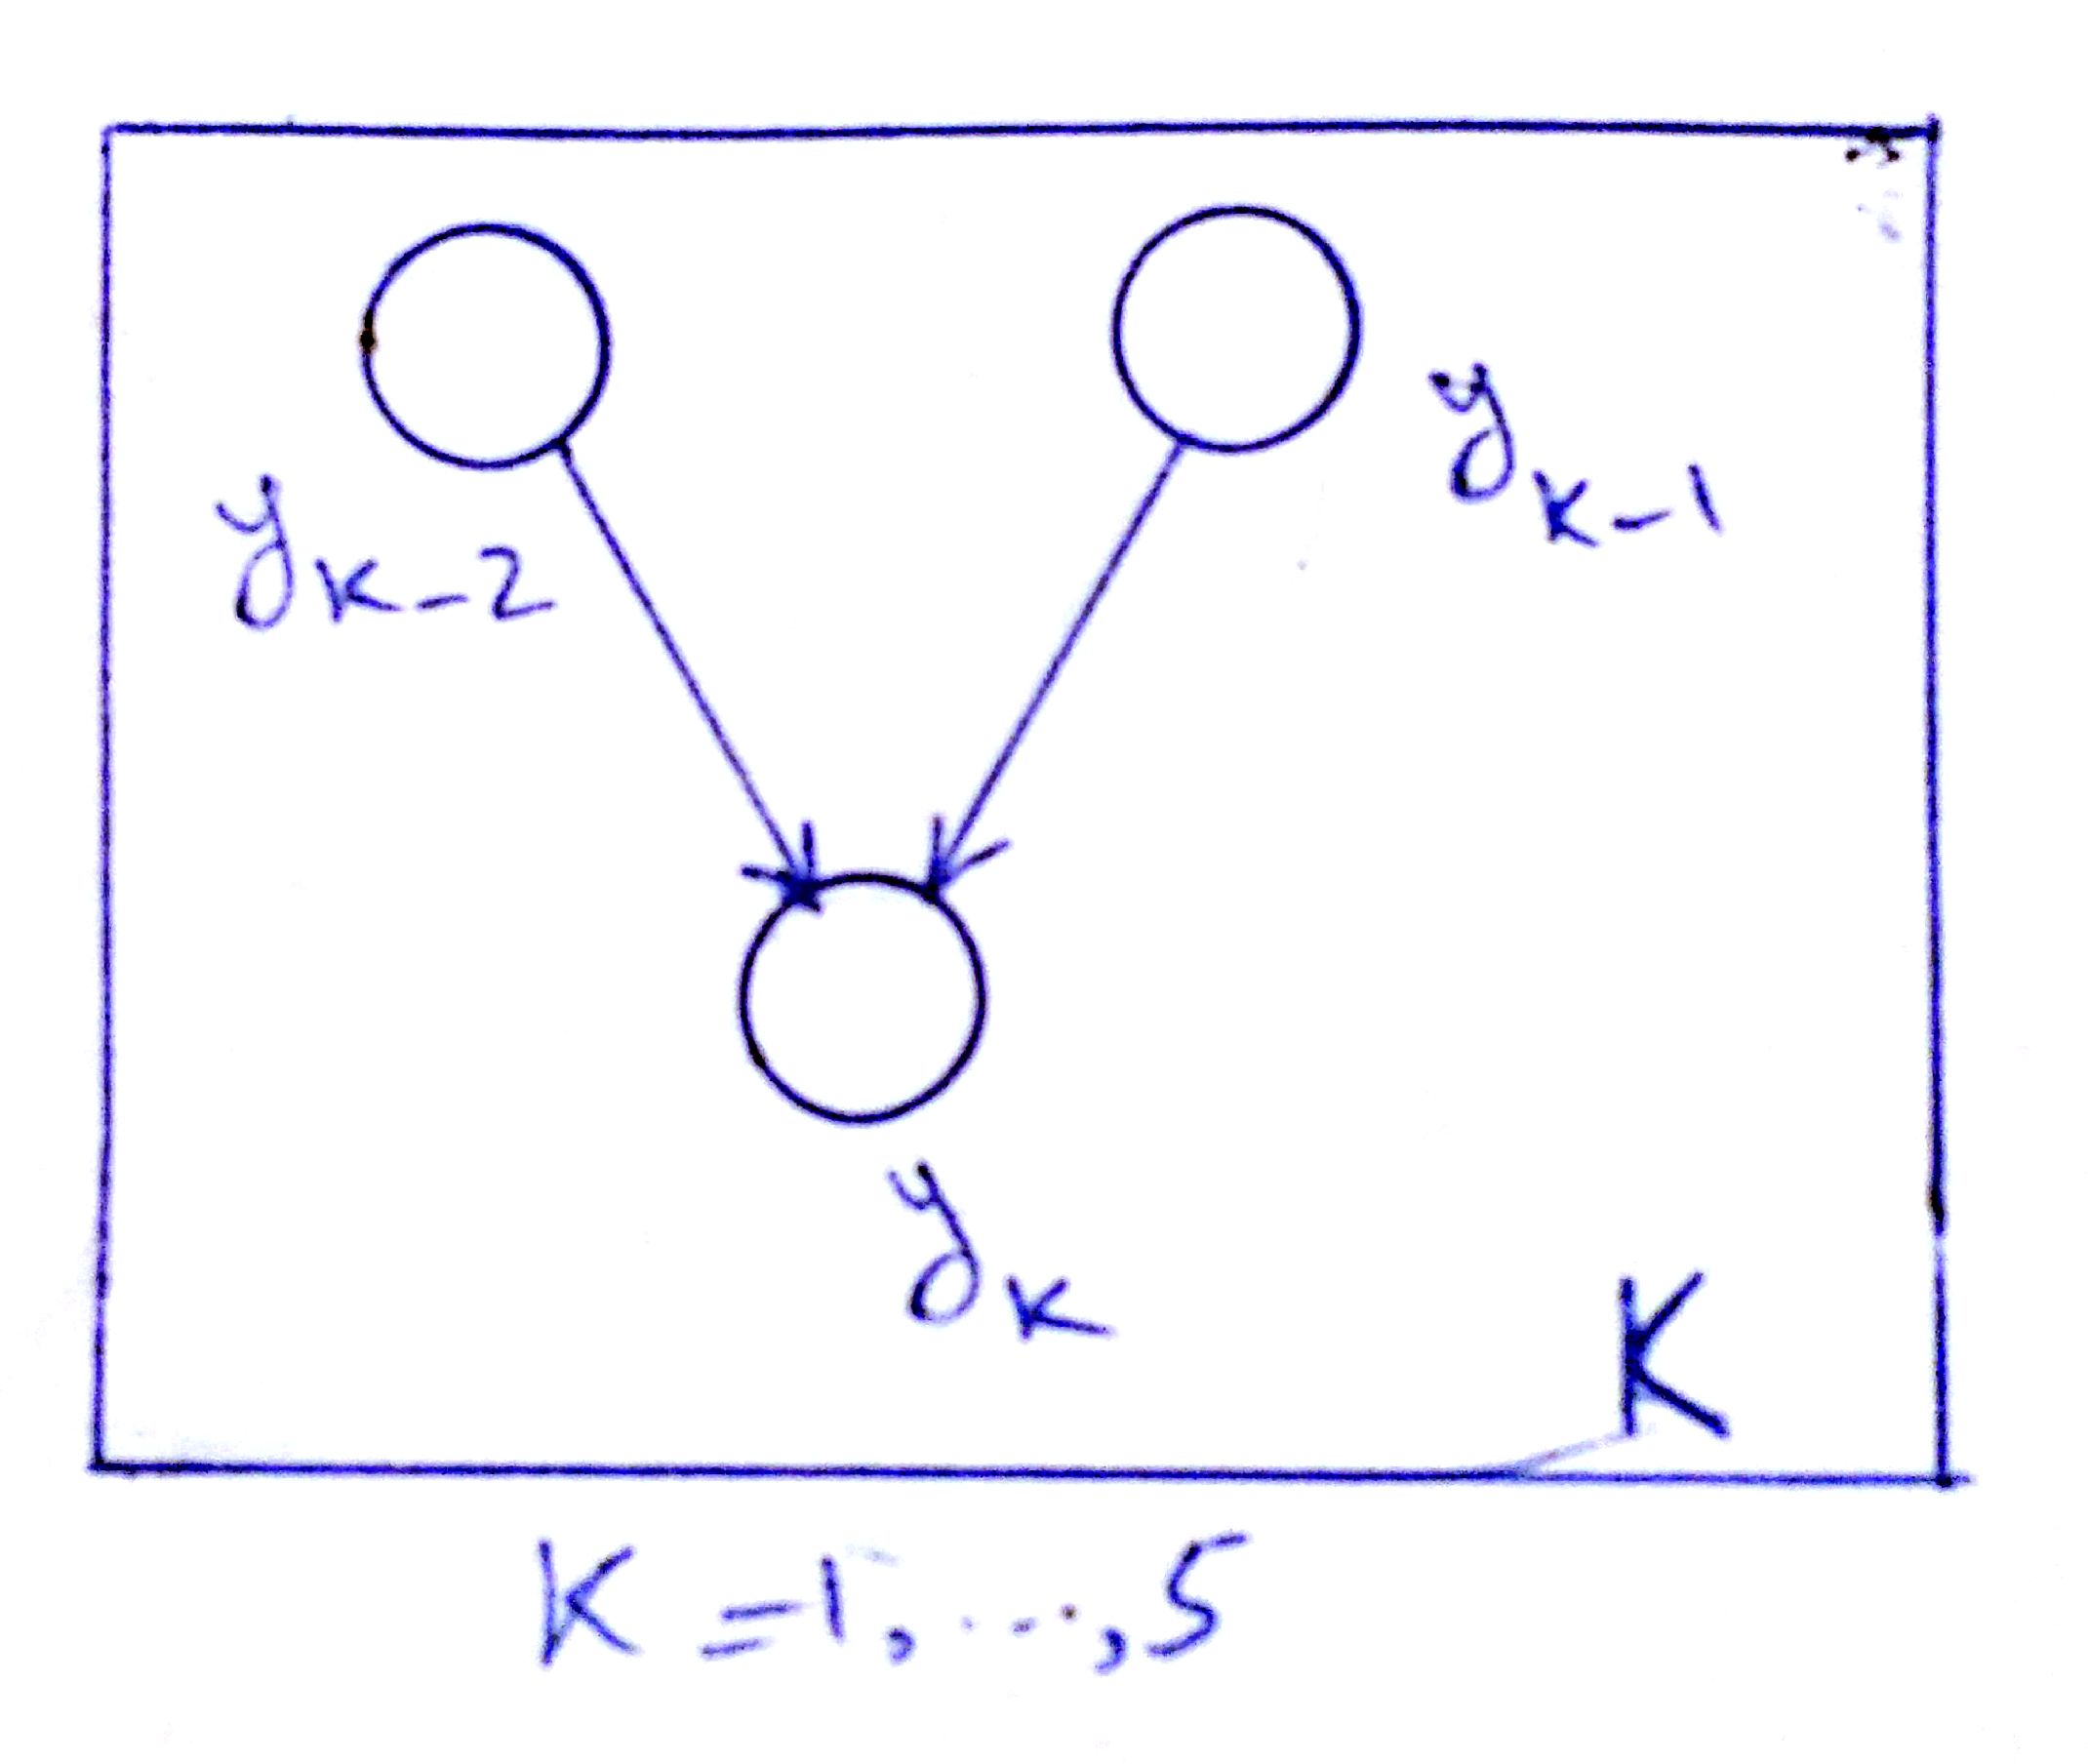
\includegraphics[width=0.3\textwidth]{question-3/3-a-i.jpg}
				\end{figure}
		}
		\subsubprob{}{
			\begin{figure}[H]
				\centering
				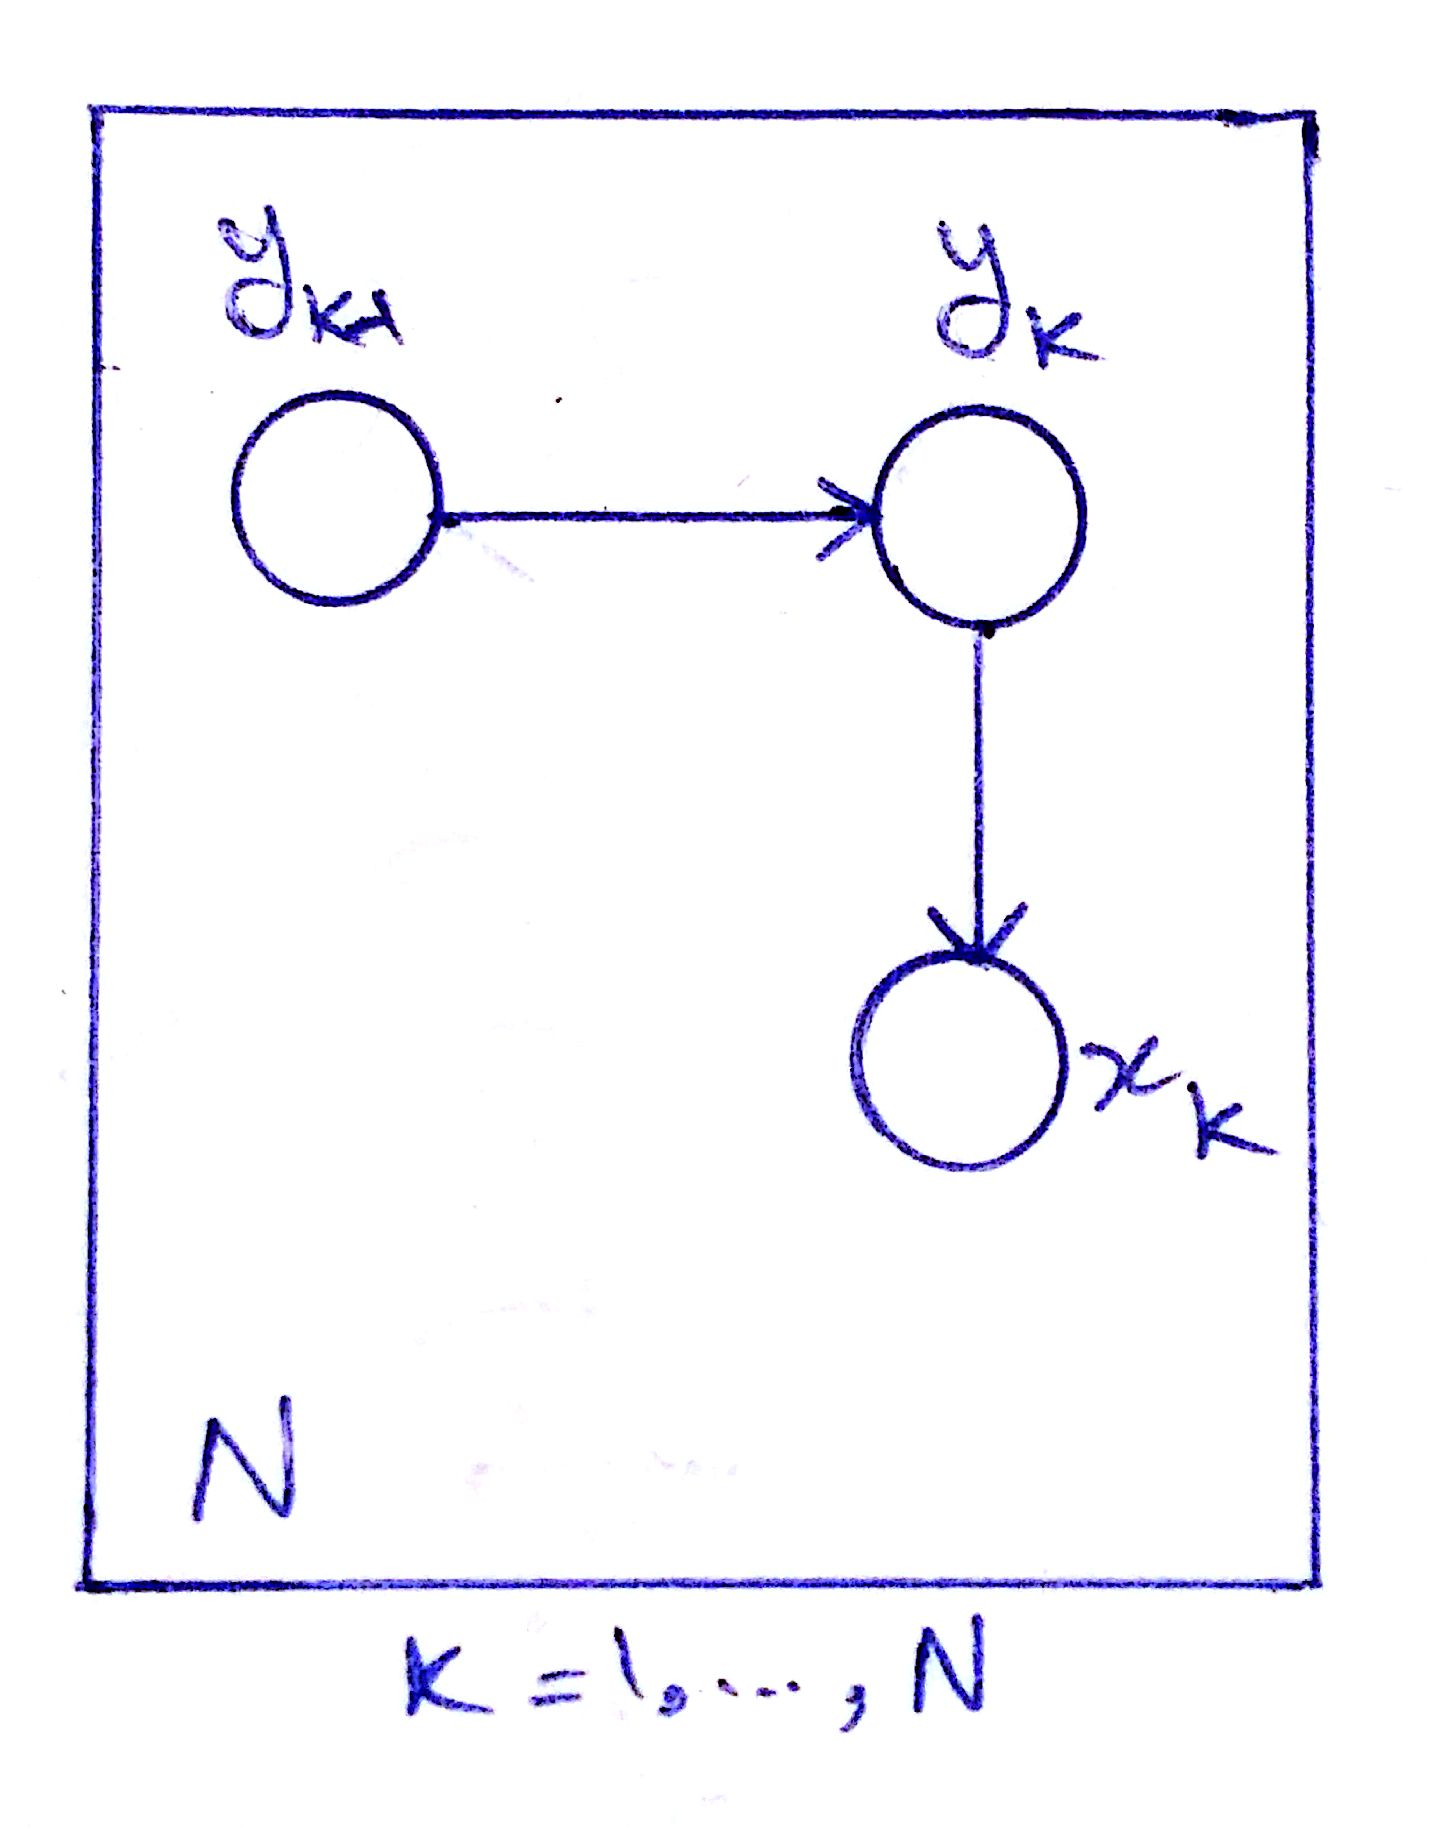
\includegraphics[width=0.3\textwidth]{question-3/3-a-ii.jpg}
			\end{figure}
		}
	}

\subprob{}{
	\begin{flalign*}
		& P(\gamma, \theta, \phi, Z) = \prod_{m=1}^{M} P(\gamma_m)P(\theta_m | \gamma_m) \prod_{n=1}^{N}P(\phi_{mn})P(Z_{mn} | \phi_{mn})\\
		& P(Z, W) = \prod_{m=1}^{M} P(z_m) \prod_{n=1}^{N}P(w_{nm} | z_m)
	\end{flalign*}
	}
	
\subprob{}{
	\begin{figure}[!ht]
		\centering
		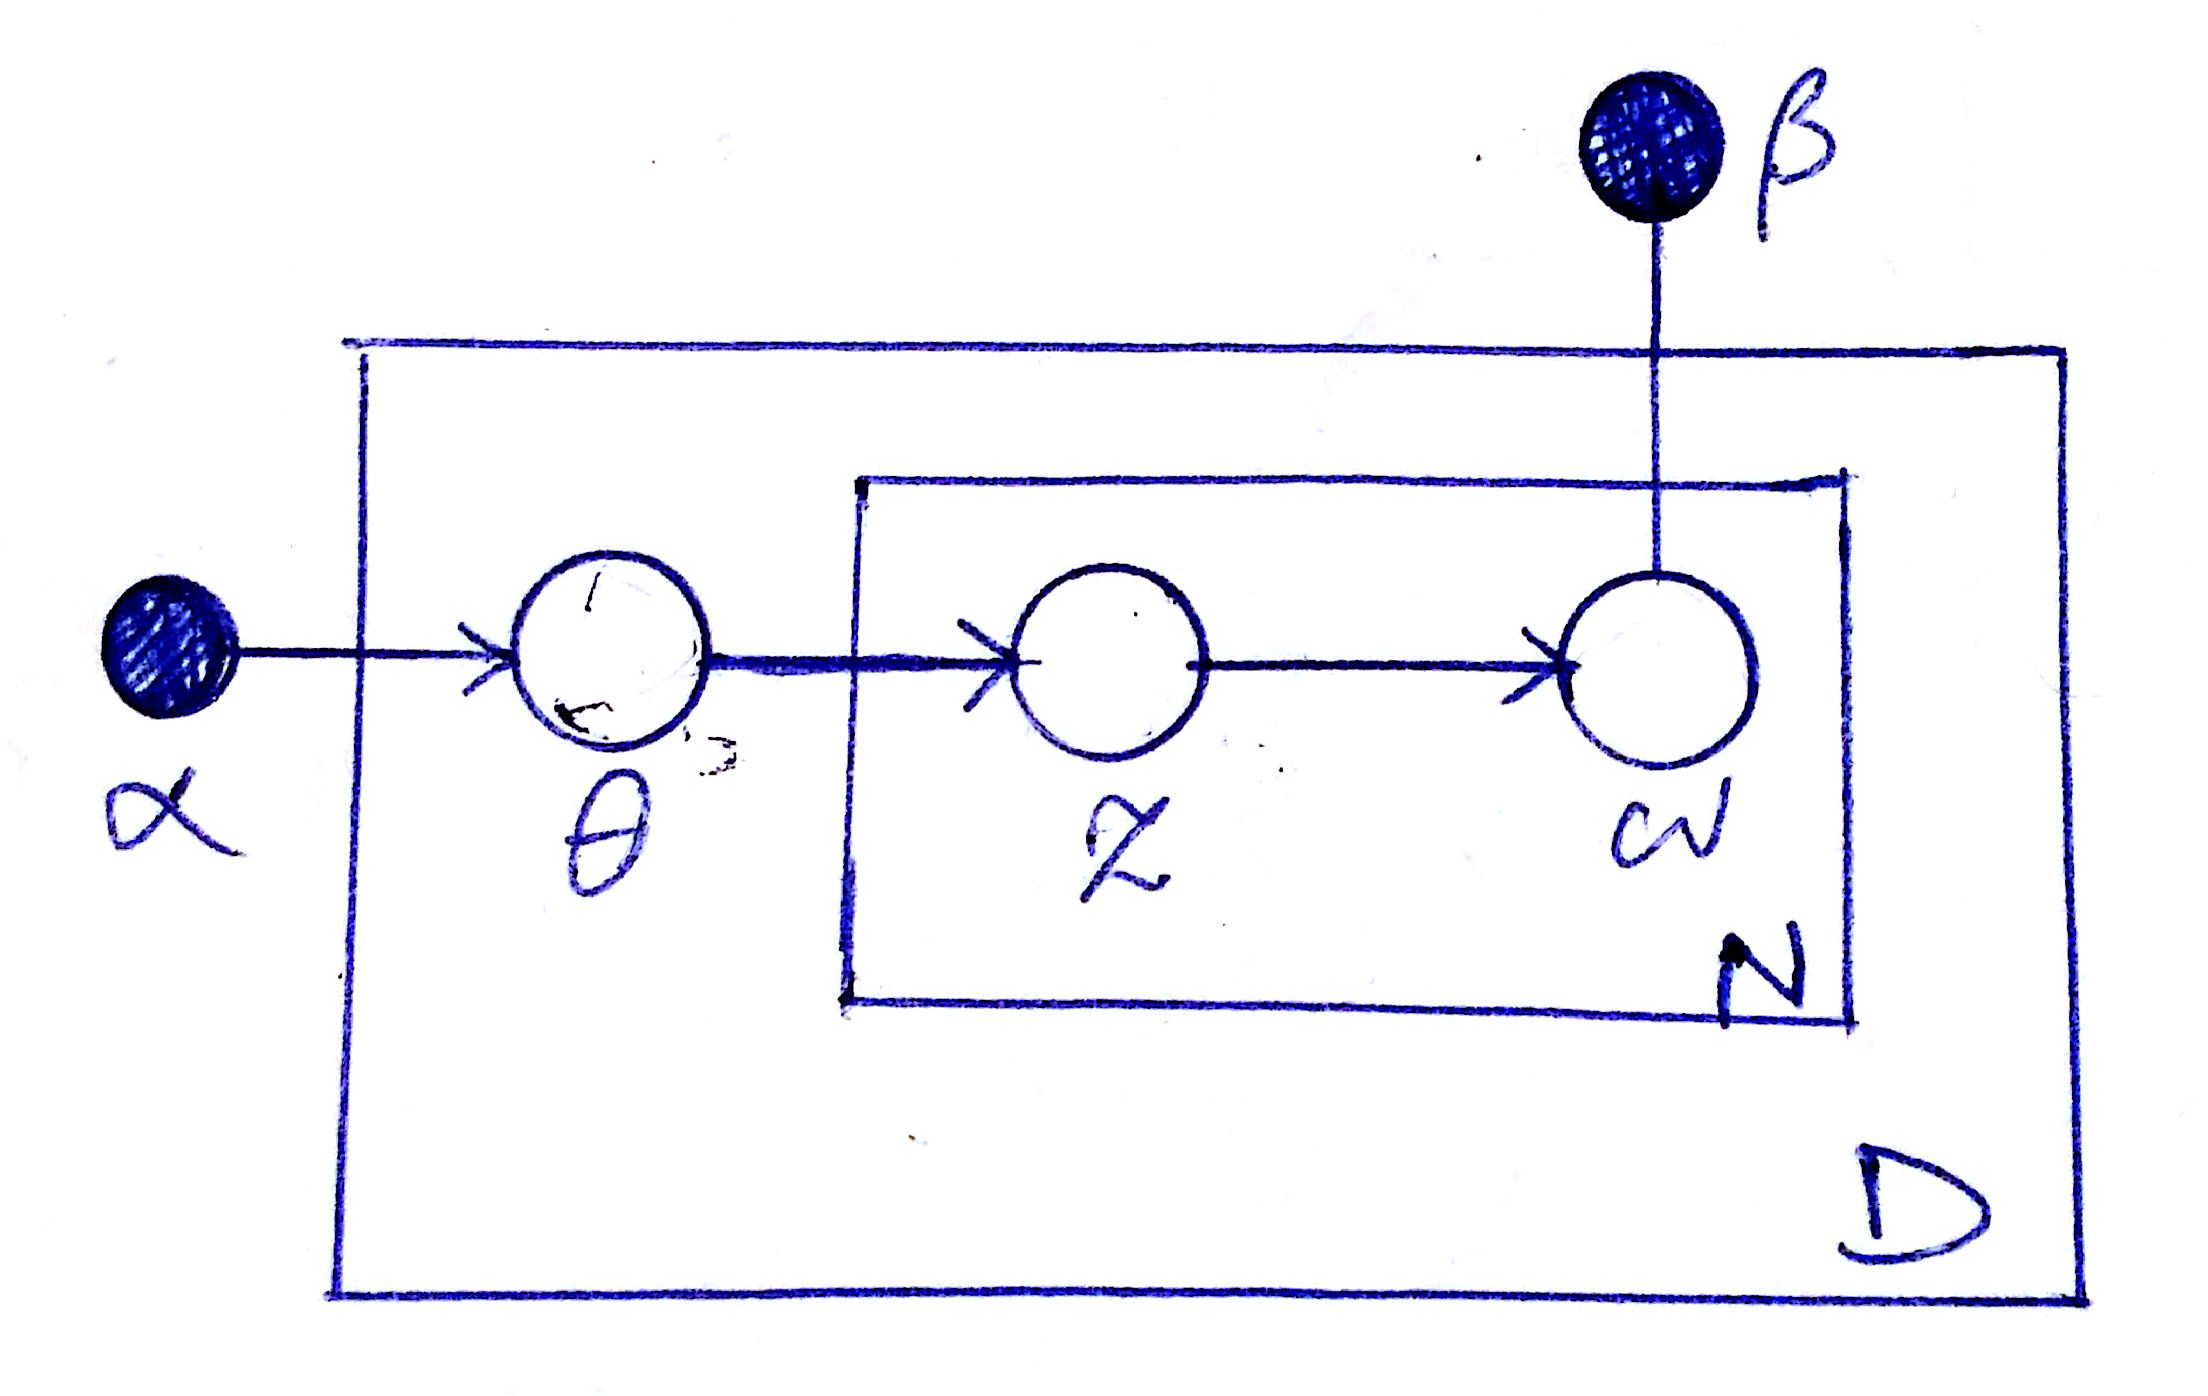
\includegraphics[width=0.4\textwidth]{question-3/3-c.jpg}
	\end{figure}
	}

}

\vspace{10cm}
\nprob{Question 4}{
	
	\subprob{}{
		\subsubprob{}
		{
	\begin{figure}[H]
		\centering
		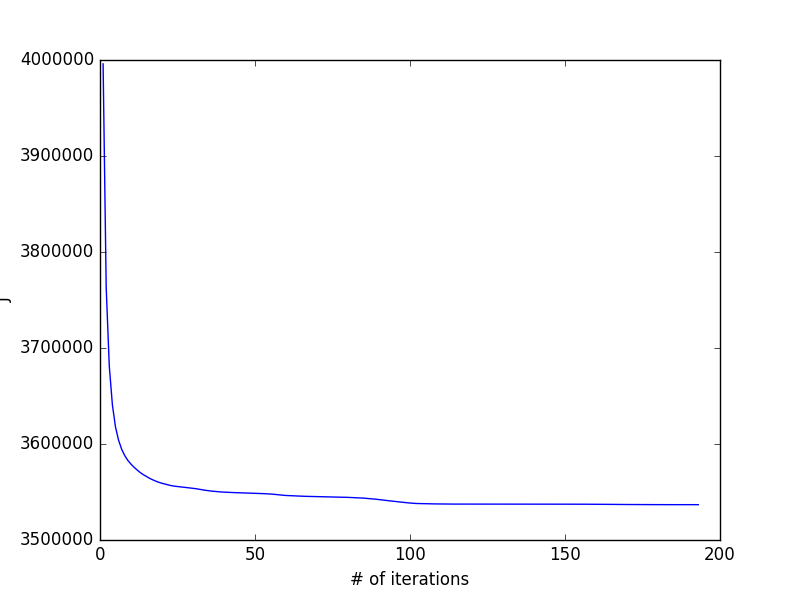
\includegraphics[width=0.4\textwidth]{question-4/plot.png}
	\end{figure}
			}
		\subsubprob{}
		{
			The boundaries where there is a change in colors are not well preserved. Each individual color region (cluster) is preserved.
		}
		\subsubprob{}
		{
			\begin{figure}[H]
				\centering
				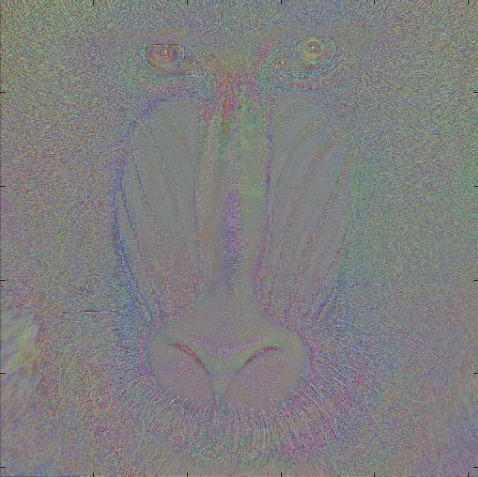
\includegraphics[width=0.4\textwidth]{question-4/mandrill-diff.png}
			\end{figure}
		}
		\subsubprob{}
		{	
			compression ratio = $\frac{\log_2 64}{24 \times 2 \times 2} = \frac{1}{16}$
		}
		\subsubprob{}
		{
			Relative mean absolute error = 0.05011	
		}
		\subsubprob{}
		{
			\lstinputlisting[language=Python, basicstyle=\scriptsize]{question-4/hw4p4-textedit.py}	
		}

	}
		
	\subprob{}{
			bpp = $\frac{\log_2 k}{M \cdot M}$
			
			compression ratio = $\frac{\frac{\log_2 k}{M \cdot M}}{24}$ = $\frac{\log_2 k}{24 M \cdot M}$	
	}

}
\vspace{30cm}
\nprob{Question 5}{
		\subprob{}{
			\begin{flalign*}
				\log f(\underline{y}|\underline{x}; \theta) &= \log \prod_{n=1}^{N} f(y_n|x_n; \theta) = \log \prod_{n=1}^{N} \sum_{k=1}^K \pi_k \phi(y; \mathbf{w}_k^T \mathbf{x} + b_k, \sigma_k^2)\\
				&= \sum_{n=1}^{N} \log \sum_{k=1}^K \pi_k \phi(y; \mathbf{w}_k^T \mathbf{x} + b_k, \sigma_k^2)
			\end{flalign*}
		}
		\subprob{}{
			\begin{flalign*}
				\log f(y_n, z_n | \mathbf{x}_n; \theta) &= \log \prod_{k=1}^{K} \pi_k \phi(y; \mathbf{w}_k^T \mathbf{x} + b_k, \sigma_k^2)^{\mathbb{I}[z_n = k]}\\
														 &= \sum_{k=1}^{K} {\mathbb{I}[z_n = k]} \log (\pi_k \phi(y; \mathbf{w}_k^T \mathbf{x} + b_k, \sigma_k^2))\\
				\log f(\underline{y}, \underline{z} | \underline{\mathbf{x}}; \theta) &= \sum_{n=1}^{N} \log f(y_n, z_n | \mathbf{x}_n; \theta)\\
				&= \sum_{n=1}^{N} \sum_{k=1}^{K} {\mathbb{I}[z_n = k]} \log (\pi_k \phi(y; \mathbf{w}_k^T \mathbf{x} + b_k, \sigma_k^2))\\
				&= \sum_{n=1}^{N} \sum_{k=1}^{K} \Delta_{nk} \log (\pi_k \phi(y; \mathbf{w}_k^T \mathbf{x} + b_k, \sigma_k^2))
			\end{flalign*}
		}
		\subprob{}{
			\begin{flalign*}
				P(z_n=k|y_n, \theta) &= \frac{P(z_n=k|\theta) P(y_n|z_n=k, \theta)}{p(y_N | \theta)} = \frac{\pi_k \phi(y_n; \mathbf{w}_k^T \mathbf{x}_n + b_k, \sigma_k^2)}{\sum_{k'=1}^{K} \pi_k' \phi(y_n; \mathbf{w}_k^T \mathbf{x}_n + b_{k'}, \sigma_{k'}^2)}\\
				Q(\theta, \theta^\mathrm{old}) &= \mathbb{E}_{\underline{z}} \left[\log f(\underline{y}, \underline{z} | \underline{\mathbf{x}}; \theta) | \underline{y},\underline{\mathbf{x}}; \theta^\mathrm{old} \right]\\
				&= \sum_{n=1}^{N} \sum_{k=1}^{K} \mathbb{E}_{\underline{z}} \left[ \Delta_{nk} \log (\pi_k \phi(y_n; \mathbf{w}_k^T \mathbf{x}_n + b_k, \sigma_k^2)) \right]\\
				&= \sum_{n=1}^{N} \sum_{k=1}^{K} \mathbb{E}_{\underline{z}} \left[ \Delta_{nk} \right] \log (\pi_k \phi(y_n; \mathbf{w}_k^T \mathbf{x}_n + b_k, \sigma_k^2))\\
				&= \sum_{n=1}^{N} \sum_{k=1}^{K} P(z_n=k|y_n, \theta) \log (\pi_k \phi(y_n; \mathbf{w}_k^T \mathbf{x}_n + b_k, \sigma_k^2))\\
				&= \sum_{n=1}^{N} \sum_{k=1}^{K} r_{nk} \log \pi_k + \sum_{n=1}^{N} \sum_{k=1}^{K} r_{nk} \log(\phi(y_n; \mathbf{w}_k^T \mathbf{x}_n + b_k, \sigma_k^2))\\
			\end{flalign*}
		}
		\subprob{}{
			\begin{flalign*}
				\Lambda(\pi, \lambda) &= Q(\theta, \theta^\mathrm{old}) + \lambda \left( \sum_{k=1}^{K} \pi_k - 1 \right) \\
				\frac{\partial \Lambda}{\partial \pi_j} &= \sum_{n=1}^{N} r_{nj} \frac{1}{\pi_j} + \lambda = 0\\
				&\sum_{n=1}^{N} r_{nk} \frac{1}{\pi_k} + \lambda = 0 \implies \sum_{n=1}^{N} r_{nk} = -\lambda \pi_k \implies \sum_{n=1}^{N} \sum_{k=1}^{K} r_{nk} = -\lambda \sum_{k=1}^{K} \pi_k \implies \lambda = -N\\
				%&\sum_{n=1}^{N} \sum_{k=1}^{K} \frac{\pi_k \phi(y_n; \mathbf{w}_k^T \mathbf{x}_n + b_k, \sigma_k^2)}{\sum_{k'=1}^{K} \pi_k' \phi(y_n; \mathbf{w}_k^T \mathbf{x}_n + b_{k'}, \sigma_{k'}^2)} = -\lambda \sum_{k=1}^{K} \pi_k \implies \lambda = -N\\
				&\sum_{n=1}^{N}r_{nk}\frac{1}{\pi_k} = N \implies \pi_k = \frac{1}{N} \sum_{n=1}^{N}r_{nk}\\
				Q(\theta, \theta^\mathrm{old}) &= \sum_{n=1}^{N} \sum_{k=1}^{K} r_{nk} \log \pi_k + \sum_{n=1}^{N} \sum_{k=1}^{K} r_{nk} \log(\phi(y_n; \mathbf{w}_k^T \mathbf{x}_n + b_k, \sigma_k^2))\\
				&= \sum_{n=1}^{N} \sum_{k=1}^{K} r_{nk} \log \pi_k + \sum_{n=1}^{N} \sum_{k=1}^{K} r_{nk} \log \left( \frac{1}{(\sigma_k \sqrt{2\pi})^d} e^{-1/2 (\frac{||\mathbf{w}_k^T \mathbf{x}_n+b_k - y_n||}{\sigma_k})^2} \right)\\
				&= \sum_{n=1}^{N} \sum_{k=1}^{K} r_{nk} \log \pi_k + \sum_{n=1}^{N} \sum_{k=1}^{K} r_{nk} \log \left( \frac{1}{(\sigma_k \sqrt{2\pi})^d} \right) + \\ &\sum_{n=1}^{N} \sum_{k=1}^{K} \frac{-r_{nk}}{2\sigma_k^2} (\mathbf{w}_k^T \mathbf{x}_n+b_k - y_n)^2\\
				&\tilde{\mathbf{w}_k}=\{\mathbf{w}_k,b_k\}, \tilde{\mathbf{x}_n}=\{\mathbf{x}_n,1\}\\
				&\text{we only care about the term dependent on }\mathbf{w}, b_k, \sigma^2 \implies\\ 
				& g(\theta, \theta^{old}) = \sum_{n=1}^{N} \sum_{k=1}^{K} \frac{-r_{nk}}{2\sigma_k^2} (\mathbf{w}_k^T \mathbf{x}_n+b_k - y_n)^2\\
				&= (\tilde{X}\tilde{\mathbf{w}_k}-y)^T R_k (\tilde{X}\tilde{\mathbf{w}_k}-y), R_k=\text{a diagonal N by N matrix where } r_{nn}=\frac{-r_{k}}{2\sigma_k^2}\\
				&\frac{\partial g(\theta, \theta^{old})}{\partial \tilde{\mathbf{w}_k}}=0 \implies\\
				&\tilde{\mathbf{w}_k^*}=(\tilde{X}^{\top}R_k\tilde{X})^{-1}\tilde{X}^{\top}R_ky = \{\mathbf{w}_k^*,b_k^*\}\\
				\frac{\partial Q(\theta, \theta^\mathrm{old})}{\partial \sigma_k^2} &= \frac{\partial}{\partial \sigma_K^2} \sum_{n=1}^{N} \sum_{k=1}^{K} r_{nk} \log \pi_k + \frac{\partial}{\partial \sigma_k^2}\sum_{n=1}^{N} \sum_{k=1}^{K} r_{nk} \log \left( \frac{1}{\sqrt{(2\pi)^d \sigma_k^2}} \right) + \\ &\frac{\partial}{\partial \sigma_k^2}\sum_{n=1}^{N} \sum_{k=1}^{K} \frac{-r_{nk}}{2\sigma_k^2} (\tilde{\mathbf{w}_k}\tilde{x}_n-y_n)^2\\
				&= \sum_{n=1}^{N} \frac{-r_{nk}}{2\sigma_k^2} + \sum_{n=1}^{N}\frac{r_{nk}}{2\sigma_k^4}(\tilde{\mathbf{w}_k}\tilde{x}_n-y_n)^2 = 0\\
				&\implies \sigma_k^2 = \frac{(\tilde{X}\tilde{\mathbf{w}_k}-y)^T R_k (\tilde{X}\tilde{\mathbf{w}_k}-y)}{r_k}
				%\nabla_{w_k,b_k} Q(\theta, \theta^\mathrm{old}) &= \begin{bmatrix}
				 %\sum_{n=1}^{N} \frac{r_{nk}(\mathbf{w}_k^T \mathbf{x}_n+b_k - y_n)\mathbf{x}_n}{\sigma_k^2}\\[1.2em]
				%\sum_{n=1}^{N} \frac{r_{nk}(\mathbf{w}_k^T \mathbf{x}_n+b_k - y_n)}{\sigma_k^2}
				%\end{bmatrix} = 0\\
				%&\implies \sum_{n=1}^N r_{nk} (\mathbf{w}_k^T\mathbf{x}_n + b_k - y_n)\mathbf{x}_n = 0, \sum_{n=1}^N r_{nk} (\mathbf{w}_k^T\mathbf{x}_n + b_k - y_n) = 0\\
				%&\implies \sum_{n=1}^N r_{nk} (\mathbf{w}_k^T\mathbf{x}_n + b_k)\mathbf{x}_n = \sum_{n=1}^N r_{nk} y_n \mathbf{x}_n, \sum_{n=1}^N r_{nk} (\mathbf{w}_k^T\mathbf{x}_n + b_k) = \sum_{n=1}^N r_{nk} y_n\\
			\end{flalign*}
		}
		\subprob{}{
			I have some bugs in my code and I ran out while dedugging :(
			
				\begin{figure}[H]
					\centering
					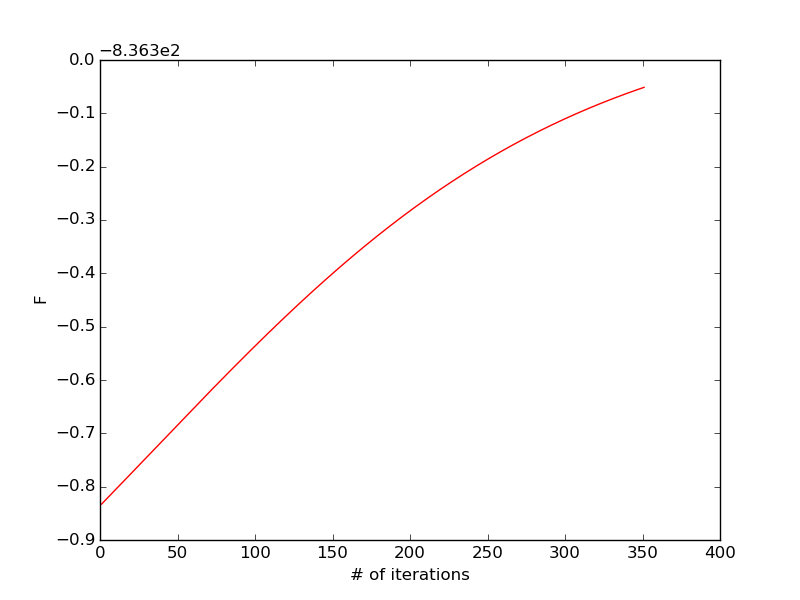
\includegraphics[width=0.6\textwidth]{question-5/plot-1.png}
				\end{figure}
				
				
				w:  [ 0.  0.]   b: [ 0.  0.] pi:  [ 0.09001366,  0.90998634] sigma:  [ 13.33434172,  13.33434172]
				
			
			\lstinputlisting[language=Python, basicstyle=\scriptsize]{question-5/hw4p5.py}
		}
}

\end{document}